
  \section{Get each page's VA with vm\_start and vm\_end}
  \begin{minted}[mathescape,
               numbersep=5pt,
               gobble=2,
               frame=lines,
               framesep=2mm]{c}
  for (vm_address = vm->vm_start;
  vm_address < vm->vm_end;
  vm_address += 0x1000)
  {
    //vm_address
  }
  \end{minted}
  
  \section{Use follow\_page with vm\_area\_struct and vm\_address to get the page}
  \begin{minted}[mathescape,
               numbersep=5pt,
               gobble=2,
               frame=lines,
               framesep=2mm]{c}
  page = follow_page(vm, vm_address, 0);
  \end{minted}
   \subsection{Use page\_to\_phys to get the physical frame addresses}
  \begin{minted}[mathescape,
               numbersep=5pt,
               gobble=2,
               frame=lines,
               framesep=2mm]{c}
  pfn = page_to_phys(page);
printk("0x%x ",pfn);
  \end{minted}

  \section{Get a file name if this file is asscociated with VMA.}
  \begin{minted}[mathescape,
               numbersep=5pt,
               gobble=2,
               frame=lines,
               framesep=2mm]{c}
          task->mm->mmap->vm_file->f_dentry->d_name.name);
  \end{minted}

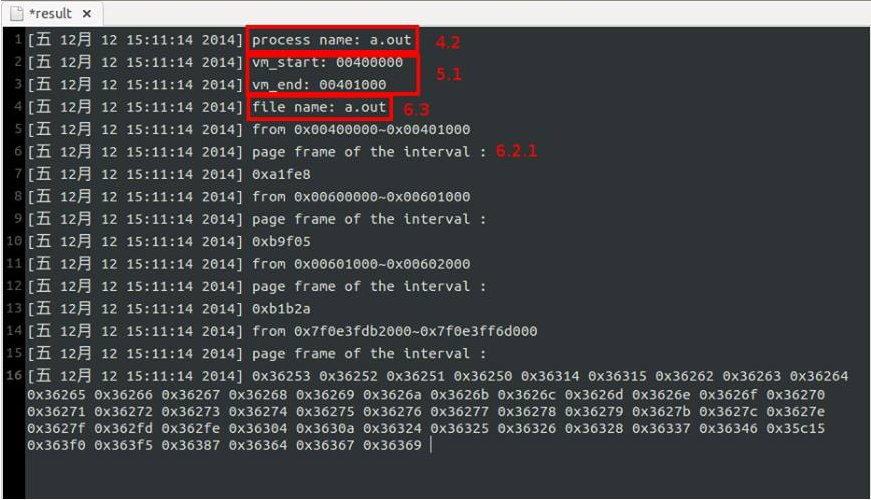
\includegraphics[scale=0.45]{pic/result.jpg}
